\chapter{Electrodinámica}
\label{cap:1}
\newpage

\section{Ecuaciones de Maxwell}

Desde el siglo XVIII, diversos científicos de la época formularon leyes que permitían entender las diversas interacciones entre los campos eléctricos y magnéticos, de las que destacan la \textit{ley de Coulomb}, la \textit{ley de Ampère}, la \textit{ley de Faraday} y la \textit{ley de Gauss}, entre otras. 

No fue hasta el año 1865 donde el físico James Clerk Maxwell (1831-1879), en su trabajo titulado \textit{A Dynamical Theory of the Electromagnetic Field} \cite{Maxwell}, resume todas las leyes anteriormente nombradas a partir elementos más fundamentales, logrando así toda la teoría electromagnética utilizando un conjunto de cuatro ecuaciones las cuales son (ver Apéndice \ref{ape:convenciones} para unidades):
\begin{center}
\begin{tabular}{l|c|c}
Nombre & Forma integral & Forma diferencial \\
\hline \hline
 & & \\
ley de Gauss & $\oiiint_{\partial \Omega} \vb{E} \cdot \mathrm{d}\vb{S} = \iiint_{\Omega} \rho \mathrm{d}V $ & $\div{\vb{E}} = 4\pi \rho$ \\
 & & \\
\hline
 & & \\
ley de Gauss magnética & $\oiiint_{\partial \Omega} \vb{B} \cdot \mathrm{d}\vb{S} = 0 $ & $\div{\vb{B}} = 0$ \\
 & & \\
\hline
 & & \\
ley de Faraday & $\oint_{\partial \Sigma} \vb{E} \cdot \mathrm{d} \vb{l} = - \pdv{}{t} \iint_{\Sigma} \vb{B} \cdot \mathrm{d} \vb{S}$ & $\curl{\vb{E}} = - \pdv{\vb{B}}{t}$ \\
 & & \\
\hline
 & & \\
ley de Ampère-Maxwell & $\oint_{\partial \Sigma} \vb{B} \cdot \mathrm{d}\vb{l} = \iint_{\Sigma} \vb{J} \cdot \mathrm{d} \vb{S} $ & $\curl{\vb{B}} = 4 \pi \vb{J} +  \pdv{\vb{E}}{t}$\\
 & $\qquad \qquad \quad + \pdv{}{t} \iint_{\Sigma} \vb{E} \cdot \mathrm{d} \vb{S}$ & \\
  & & 
\end{tabular} 
\end{center}

La \textit{ley de Gauss} describe la relación que existe entre el campo eléctrico y las cargas eléctricas que lo generan, más concretamente, nos dice si las líneas de campo son salientes o entrantes (ver figura \ref{fig:2}) dependiendo si la fuente de carga que lo genera posee carga neta $Q$ positiva o negativa respectivamente.
\begin{figure}[!ht]
\centering
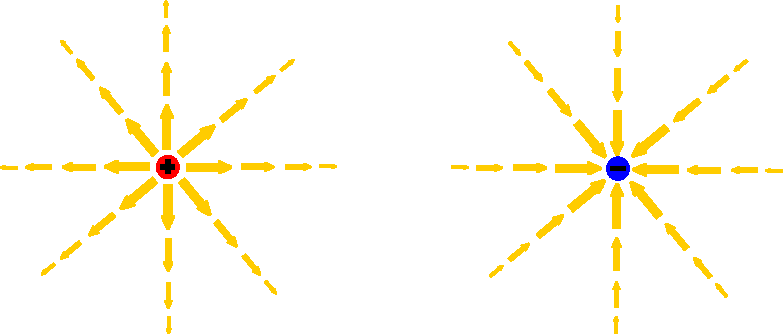
\includegraphics[scale=1]{images/sumidero-fuente.pdf}
\caption[Ley de Gauss]{Sumideros y fuentes respectivamente.}
\label{fig:2}
\end{figure}

La \textit{ley de Gauss magnética} nos dice que no existen monopolos magnéticos, los cuales serían los análogos magnéticos de las cargas. Dicho de otro modo, una superficie cerrada ubicada en cualquier punto del espacio siempre tendrá un flujo de campo magnético neto igual a 0. Esto puede entenderse al ver la figura \ref{fig:3} en donde se intenta esquematizar un dipolo magnético, y en particular, se puede observar que cada linea de campo siempre intercepta la superficie cerrada en dos ocasiones, una desde el polo positivo hacia fuera de la superficie (saliendo) y otra desde fuera de la superficie hasta el polo negativo (entrando), dando como resultado un flujo de campo magnético nulo.
\begin{figure}[!ht]
\centering
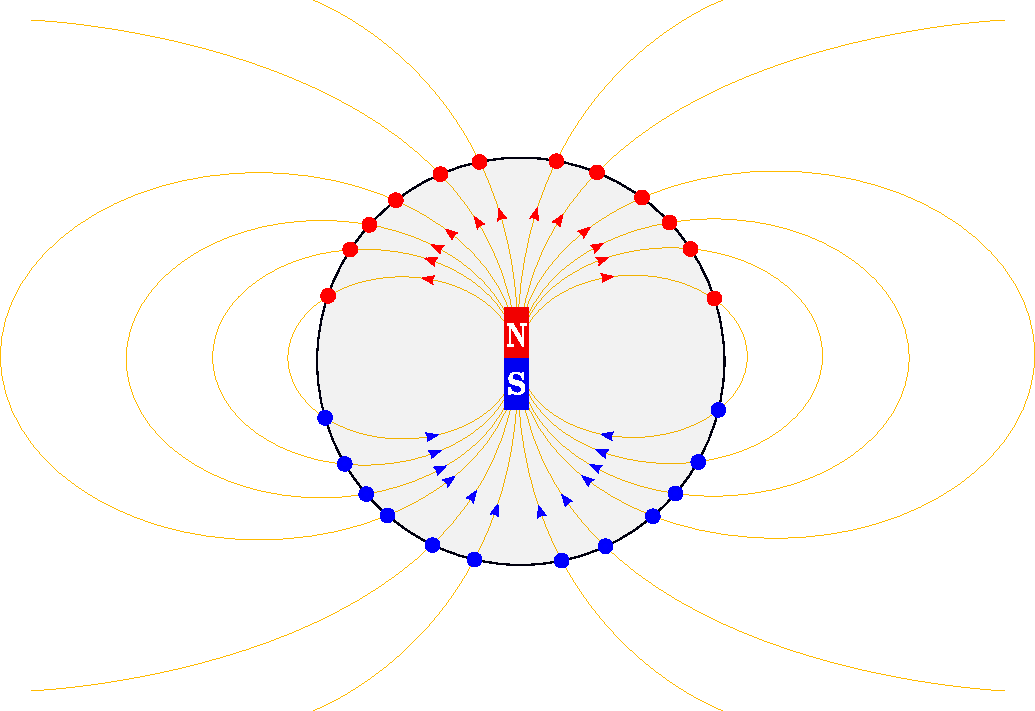
\includegraphics[scale=0.7]{images/ley-de-gauss-magnetismo.pdf}
\caption[Ley de Gauss para magnetismo]{Dipolo magnético dentro de superficie cerrada.}
\label{fig:3}
\end{figure}

La \textit{ley de Faraday} nos explica cómo funcionan los efectos de inducción magnética, esto quiere decir que si tengo un campo magnético variando en el tiempo, a su vez, éste inducirá un campo eléctrico.  Y la \textit{ley de Ampère-Maxwell} complementa lo anterior diciendo que un campo eléctrico variando en el tiempo inducirá un campo magnético. De esta forma podemos hacer notar que no solo las cargas e imanes son los culpables de influir en los campos eléctricos y magnéticos respectivamente, si no que también una fuente de campo magnético puede ser un campo eléctrico variando en el tiempo y viceversa.

Una de las importantes consecuencias de estas ecuaciones es que ellas implican la \textit{ley de conservación de la carga eléctrica} o \textit{ecuación de continuidad}. En particular, si calculamos la divergencia del rotor del campo magnético obtenemos que
\begin{align}
\div{\curl{\vb{B}}} &= \div{ \left( \pdv{\vb{E}}{t} + 4\pi \vb{J} \right) }\\
&= 4\pi \pdv{\rho}{t} + 4\pi \div{\vb{J}}\\
&= 0,
\end{align}
obteniendo la ecuación de continuidad.

\section{Formulación covariante}

En el año 1905, el físico alemán Albert Einstein (1879-1955) presentó por primera vez en su trabajo titulado \textit{Zur Elektrodynamik Bewegter Körper} \cite{Einstein} (``Sobre la electrodinámica de los cuerpos en movimiento'') su Teoría Especial de la Relatividad basada en dos postulados, los cuales son:
\begin{itemize}
\item[1)] Las leyes de la Física son invariantes en todos los sistemas de referencia inerciales.
\item[2)] La velocidad de la luz en el vacío es igual para todos los observadores, independiente del movimiento de la fuente de luz.
\end{itemize}

Pese a las inconsistencias de su teoría con la mecánica newtoniana, el trabajo de Einstein logró solucionar uno de los mayores problemas de la época, pero antes de explicarlo es necesario ponernos en contexto.

Como se muestra anteriormente, Maxwell logra unificar con sus ecuaciones toda la teoría electromagnética en 4 ecuaciones el año 1865. Sin embargo dichas ecuaciones presentaban un problema, y era que estas no eran invariantes bajo transformaciones de Galileo. Esto quiere decir que, si consideramos un observador inercial $O$ y otro observador $O'$ moviéndose con velocidad constante $\vb{v}$ respecto a $O$, las ecuaciones de Maxwell respecto a $O'$ son diferentes y, por ende, implicaría la existencia de observadores privilegiados en el Universo, lo cual va en contra del primer principio mostrado anteriormente. 

Bajo esta lógica, las ecuaciones de Maxwell debieran ser erróneas, pero en todos los experimentos en los cuales se les ponía a prueba, no se logra evidenciar inconsistencias entre las ecuaciones y los resultados experimentales, dando a entender que las predicciones hechas por dichas ecuaciones eran correctas. El problema era simple, las ecuaciones de Maxwell eran incorrectas o las transformaciones que se utilizaban para relacionar los observadores $O$ y $O'$ lo eran.

No fue hasta que Einstein presenta su teoría en donde muestra las transformaciones de Lorentz como medio para relacionar observadores inerciales, y cómo estas mantienen la invariancia de las ecuaciones de Maxwell.

Al pasar los años, varios experimentos han logrado corroborar la teoría de Relatividad Especial (SR por sus siglas en inglés), prediciendo así efectos de los cuales antes no se conocía su existencia, como por ejemplo la dilatación temporal.

Por otro lado, y pese a que la teoría de SR permitía solucionar el problema de las ecuaciones de Maxwell, también era necesario asegurar que la teoría electromagnética fuera compatible con los principios que Einstein postuló en su teoría. Por esta razón se define el \textit{tensor de Faraday}
\begin{equation}
F^{\mu \nu} := \mqty*(
0 & -E^x & -E^y & -E^z \\
E^x & 0 & -B^z & B^y \\
E^y & B^z & 0 & -B^x \\
E^z & -B^y & B^x & 0 \\ 
),
\end{equation}
lo cual permite reescribir las ecuaciones inhomogéneas de Maxwell (la \textit{ley de Gauss} y la \textit{ley de Ampère-Maxwell}) de una forma más compacta como
\begin{equation}
\label{eq:1}
\partial_{\mu} F^{\mu \nu} = 4\pi J^{\nu},
\end{equation}
donde $J^{\mu} := \rho_0 u^{\mu}$ es la 4-densidad de corriente, $\rho_0$ es la densidad de carga respecto a un sistema de referencia inercial con la fuente y $u^{\mu}$ es la 4-velocidad de la fuente.

Así mismo, también es posible reescribir las ecuaciones homogéneas de Maxwell como
\begin{equation}
\label{eq:2}
\partial_{[\mu} F_{\nu \lambda]} = 0.
\end{equation}

Condensando así las cuatro ecuaciones de Maxwell presentadas anteriormente en \eqref{eq:1} y \eqref{eq:2}.

\subsection{Tensor dual}

Otra forma de escribir \eqref{eq:2} con el fin de que se asemeje más a \eqref{eq:1}, es introduciendo la definición del tensor dual. 

Sea $A^{\mu \nu}$ un tensor bajo transformaciones generales de coordenadas, se define el dual como
\begin{equation}
\dual{A}^{\mu \nu} := \frac{1}{2} \epsilon^{\mu \nu \lambda \rho} A_{\lambda \rho},
\end{equation}
donde $\epsilon^{\mu \nu \lambda \rho}$ es el pseudo-tensor de Levi-civita definido en el Apéndice \ref{ape:convenciones}.

También notamos que es posible obtener la relación inversa, es decir, a partir del tensor dual recuperar el tensor original
\begin{equation}
A^{\mu \nu} = -\frac{1}{2} \epsilon^{\mu \nu \lambda \rho} \dual{A}_{\lambda \rho}.
\end{equation}

Así el tensor electromagnético dual es
\begin{equation}
\label{eq:3}
\dual{F}^{\mu \nu} := \mqty*(
0 & -B^x & -B^y & -B^z \\
B^x & 0 & -E^z & E^y \\
B^y & E^z & 0 & -E^x \\
B^z & -E^y & E^x & 0 \\ 
),
\end{equation}
lo que, en este caso, es equivalente a reemplazar $\vb{E}$ por $\vb{B}$ y viceversa.

Finalmente, de las ecuaciones homogéneas de Maxwell pueden ser escritas usando el tensor dual como
\begin{equation}
\partial_{\mu} \dual{F}^{\mu \nu} = 0,
\end{equation}
siendo esta forma muy similar a \eqref{eq:1}.

\section{Fuerzas de marea}
\label{sec:1}

En mecánica newtoniana, usamos el término \textbf{fuerzas de marea} para referirnos a los efectos de las inhomoeneidades del campo gravitacional (el cual produce diferentes aceleraciones en masas de prueba ubicadas en diferentes puntos del espacio). Por ejemplo, si consideramos dos masas puntuales de prueba, en caída libre y separadas una distancia infinitesimal, un observador en caída libre junto a ellas apreciará que, mientras están cayendo, estas se acercan entre sí experimentando una aparente fuerza entre ellas.

Siguiendo el ejemplo anterior, sean $\vb{x}_1$ y $\vb{x}_2$ las posiciones de ambas masas de prueba, y tales que $\vb{x}_2 = \vb{x}_1 + \delta \vb{x}$, la aceleración con la que ambas masas caen son $g_i[\vb{x}_1]$ y $g_i[\vb{x}_2]$ respectivamente (ver figura \ref{fig:4}). 
\begin{figure}[h!]
\centering
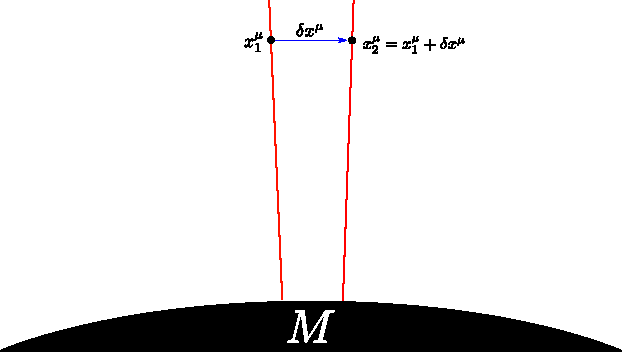
\includegraphics[scale=1.2]{images/desvio.pdf}
\caption[Esquema de desvío]{Esquema de los efectos de las inhomogeneidades del campo gravitacional.}
\label{fig:4}
\end{figure}

En particular, la aceleración de la segunda masa es
\begin{equation}
g_i[x+\delta x] = g_i[x] + \left( \partial_j g_i[x] \right) \delta x_j + \mathcal{O}(x^2).
\end{equation}

Podemos definir la aceleración relativa entre ambas masas como
\begin{equation}
\delta g_i = g_i[x+\delta x] - g_i[x] \approx \left( \partial_j g_i[x] \right) \delta x_j,
\end{equation}
y, como la aceleración a su vez es definida como la segunda derivada temporal de la posición, la ecuación anterior puede ser escrita como
\begin{equation}
\label{eq:122}
\dv[2]{ }{t} \delta x_i = (\partial_j g_i) \delta x_j.
\end{equation}

Como podemos ver, todo esto nace del hecho que el campo gravitacional no es igual en todos los puntos del espacio, lo mismo ocurre con el campo electromagnético. Si consideramos dos cargas con el mismo cociente $q/m$ separadas infinitesimalmente, siendo afectadas por la presencia de un campo electromagnético externo, y descritas por el mismo parámetro $\tau$. Entonces las fuerzas que afectan a ambas cargas son, respectivamente,
\begin{equation}
\label{eq:4}
\dv[2]{x_1^{\mu}}{\tau} = \frac{q}{m} F^{\mu}_{\ \nu}[x_1] \dv{x_1^{\nu}}{\tau}, \qquad 
\dv[2]{x_2^{\mu}}{\tau} = \frac{q}{m} F^{\mu}_{\ \nu}[x_2] \dv{x_2^{\nu}}{\tau},
\end{equation}
donde $x_1^{\mu}$ y $x_2^{\mu}$ son las curvas descritas por la primera y segunda carga respectivamente. Al expandir el tensor de Faraday hasta primer orden en serie de Taylor, se obtiene que
\begin{equation}
F^{\mu}_{\ \nu}[x_2] = F^{\mu}_{\ \nu}[x_1 + \delta x] \approx F^{\mu}_{\ \nu}[x_1] + \partial_{\sigma} F^{\mu}_{\ \nu}[x_1] \delta x^{\sigma}.
\end{equation}

Así 
\begin{equation}
\label{eq:5}
\dv[2]{x_2^{\mu}}{\tau} = \dv[2]{ }{\tau} \left( x_1^{\mu} + \delta x^{\mu} \right) = \frac{q}{m} \left( F^{\mu}_{\ \nu}[x_1] + \partial_{\sigma} F^{\mu}_{\ \nu}[x_1] \delta x^{\sigma} \right) \dv{ }{\tau} \left( x_1^{\nu} + \delta x^{\nu} \right),
\end{equation}
y reemplazando \eqref{eq:5} en la definición $\delta x^{\mu} := x_2^{\mu} - x_1^{\mu}$, se obtiene que
\begin{equation}
\dv[2]{ }{\tau} \delta x^{\mu} = \frac{q}{m} \left[ F^{\mu}_{\ \nu} \dv{ }{\tau} \delta x^{\nu} + \partial_{\gamma} F^{\mu}_{\ \nu} u^{\nu} \delta x^{\gamma} + \partial_{\gamma} F^{\mu}_{\ \nu} \delta x^{\gamma} \dv{ }{\tau} \delta x^{\nu} \right].
\end{equation}

Por último, si se asume que
\begin{equation}
\left| \dv{\tau} \delta x^{\mu} \right| \ll |u^{\mu}|,
\end{equation}
es decir, la 4-velocidad de las cargas definida como $u^{\mu}_{1,2} := \mathrm{d}x^{\mu}_{1,2}/\mathrm{d}\tau $ son aproximadamente iguales, se tiene que
\begin{equation}
\label{eq:6}
\dv[2]{ }{\tau} \delta x^{\mu} = \frac{q}{m} \left( \partial_{\gamma} F^{\mu}_{\ \nu} \right) u^{\nu} \delta x^{\gamma},
\end{equation}
que representa las inhomogeneidades del campo electromagnético y, como es de esperar, presenta una clara similitud con \eqref{eq:122}. Esto es por que tanto \eqref{eq:122} como \eqref{eq:6} son la aceleración relativa entre ambas partículas de prueba, el primero en el contexto de Relatividad General y el segundo en el de la teoría electromagnética clásica.

\section{Expansión multipolar}
\label{sec:2}

Si consideramos una distribución compacta de carga y corriente respectivamente, podemos hacer uso del método de expansión multipolar para calcular los valores del potencial escalar y vectorial en todos los puntos del espacio. Para esto es necesario describir todos los puntos de la distribución en cuestión respecto un punto de referencia $O$ (usualmente elegido en un punto al interior de esta). Así, para un punto lejano $\vb{x}$ (es decir, a una distancia mucho más grande que el tamaño de la distribución), escribimos los potenciales como una suma infinita de términos descritos en términos de $\vb{x}'$ (los cuales representan los puntos de la distribución respecto al punto $O$) y finalmente, bajo la hipótesis de que $|\vb{x}| \gg |\vb{x}'|$, introducimos la definición de los momentos multipolares para cada elemento de la expansión.
\begin{figure}[h!]
\centering
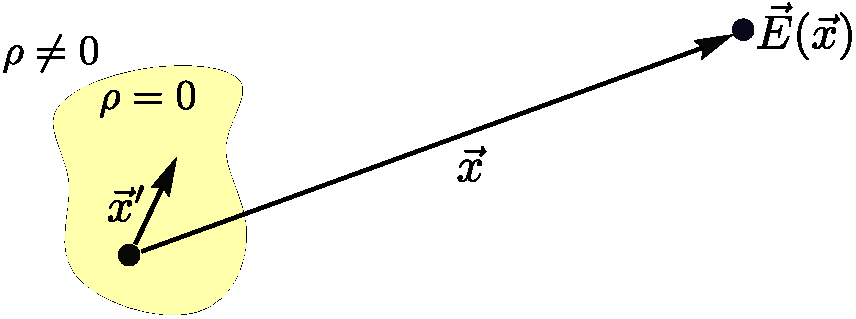
\includegraphics[scale=1]{images/multipolar.pdf}
\caption[Expansión multipolar electromagnética]{Expansión multipolar en electromagnetismo.}
\end{figure}

Para una distribución electroestática de carga, sabemos que el potencial escalar de dicha carga viene dado por
\begin{equation}
\Phi(\vb{x}) = \int_{\Omega} \frac{\rho(\vb{x})}{|\vb{x} - \vb{x}'|} d^3x,
\end{equation}
donde $\Omega$ son los puntos que componen la distribución. Como podemos observar, es necesario resolver la integral la cual, en general, es complicado desde un punto de vista matemático. 

No obstante, haciendo uso de la expansión en serie de Taylor podemos notar que
\begin{align}
\frac{1}{|\vb{x} - \vb{x}'|} &= \frac{1}{|\vb{x}|} - x'_a \partial_a \left( \frac{1}{|\vb{x} - \vb{x}'|} \right)_{x'=0} + \frac{1}{2!} x'_a x'_b \partial_a \partial_b \left( \frac{1}{|\vb{x} - \vb{x}'|} \right)_{x'=0} + \dots,\\
&= \frac{1}{|\vb{x}|} - x'_a \partial_a \frac{1}{|\vb{x}|} + \frac{1}{2!} x'_a x'_b \partial_a \partial_b \frac{1}{|\vb{x}|} + \dots,\\
&= \frac{1}{r}  - x'_a \partial_a \frac{1}{r} + \frac{1}{2!} x'_a x'_b \partial_a \partial_b \frac{1}{r} + \dots,\\
&= \sum_{n=0}^{\infty} \frac{(-1)^n}{n!} x'_{a_1} \dots x'_{a_n} \partial_{a_1} \dots \partial_{a_n} \frac{1}{r},
\end{align}
y así
\begin{equation}
\Phi(\vb{x}) = \sum_{n=0}^{\infty} Q_{a_1 a_2 \dots a_n} \partial_{a_1} \partial_{a_2} \dots \partial_{a_n} \frac{1}{r},
\end{equation}
donde $Q_{i_1 i_2 \dots i_n}$ son los momentos multipolares eléctricos definidos como
\begin{equation}
Q_{a_1 a_2 \dots a_n} := \int_{\Omega} x_{a_1} x_{a_2} \dots x_{a_n} \rho(\vb{x}) d^3x.
\end{equation}

Usando la misma idea podemos definir los momentos multipolares magnéticos
\begin{equation}
M_{a_1 a_2 \dots a_n b} := \int_{\Omega} x_{a_1} x_{a_2} \dots x_{a_n} J_b(\vb{x}) \  d^3x,
\end{equation}
y así reescribir el potencial vectorial como
\begin{equation}
A_a(\vb{x}) = \sum_{n=0}^{\infty} \frac{(-1)^n}{n!} M_{a_1 a_2 \dots a_n b} \partial_{a_1} \partial_{a_2} \dots \partial_{a_n} \frac{1}{r}.
\end{equation}

Podemos entender lo anterior como dos expansiones multipolares diferentes, una para el caso eléctrico y otra para el caso magnético. Sin embargo, es posible reformular dichas expansiones a fin de introducir el tensor de Faraday y con ello obtener una versión relativista para dicha expansión.

A partir de la fuerza de Lorentz podemos ver que
\begin{equation}
\label{eq:106}
F^{\mathrm{EM}}_{\mu} = \int_{\Omega} F_{\mu \nu}(x') J^{\nu}(x') \mathrm{d}V',
\end{equation}
y expandiendo en serie de Taylor el tensor de Faraday se obtiene que
\begin{equation}
\label{eq:107}
F_{\mu \nu}(x') = F_{\mu \nu}(X + \delta x) = F_{\mu \nu}(X) +  \partial_{\gamma} F_{\mu \nu}(X) \delta x^{\gamma} +  \frac{1}{2} \partial_{\xi} \partial_{\gamma} F_{\mu \nu}(X) \delta x^{\gamma} \delta x^{\xi} + \dots,
\end{equation}
donde $X$ denota la línea de mundo de $O$ y $\delta x$ la diferencia de coordenadas de una vecindad de puntos respecto de $O$. 

Así hasta primer orden, la ecuación \eqref{eq:106} se transforma en
\begin{equation}
\label{eq:121}
F^{\mathrm{EM}}_{\mu} = F_{\mu \nu}(X) \int_{\Omega} J^{\nu} \mathrm{d}V' + \partial_{\gamma} F_{\mu \nu}(X) \int_{\Omega} J^{\nu} \delta x^{\gamma} \mathrm{d}V'.
\end{equation}

Definiendo los momentos multipolares como
\begin{align}
\label{eq:108}
M^{\mu} &:= \int_{\Omega} J^{\mu} \mathrm{d}V',\\
\label{eq:109}
M^{\mu \nu} &:= \int_{\Omega} J^{\mu} \delta x^{\nu} \mathrm{d}V',\\
M^{\mu \nu \gamma} &:= \int_{\Omega} J^{\mu} \delta x^{\nu} \delta x^{\gamma} \mathrm{d}V',\\
\vdots & \qquad \vdots \nonumber \\
M^{\mu \nu \dots \gamma} &:= \int_{\Omega} J^{\mu} \delta x^{\nu} \dots \delta x^{\gamma} \mathrm{d}V',
\end{align}
se puede re-escribir \eqref{eq:121} como
\begin{equation}
F^{\mathrm{EM}}_{\mu} = F_{\mu \nu}[X] M^{\nu} + \left( \partial_{\gamma} F_{\mu \nu}[X] \right) M^{\nu \gamma}.
\end{equation}


\subsection{Dipolo magnético}

Se define un dipolo magnético como una distribución idealizada que solo posee momento 2-polar no-nulo, es decir $M^{\mu \nu} \neq 0$, $M^{\mu} = 0$ y $M^{\mu \nu \dots \gamma} = 0$.

Podemos calcular la fuerza que experimenta un dipolo magnético producto de un campo magnético externo independiente del tiempo, es decir $\vb{E}=0$. El campo externo es descrito por el tensor de Faraday, mientras que los momentos multipolares describen el dipolo magnético, y la fuerza de Lorentz representa la fuerza que ejerce el campo magnético externo sobre el dipolo.

Al estar considerando $X^{\mu}$ como las coordenadas de la línea de mundo de referencia para describir los elementos de la distribución en cuestión, es necesario notar que al introducir la componente temporal en la formulación, es necesario fijar un tiempo en el cual se realiza esta descripción, dando a entender que para un instante de tiempo $t_0$, la componente $X^0$ siempre igual a las componentes $x^0$ de los puntos que conforman la vecindad de $O$, deduciendo que $\delta x^0 = 0$, lo cual al introducir en \eqref{eq:109} implica que $M^{\mu 0} = 0$, y al ser un dipolo magnético, entonces $M^{(\mu \nu)} = 0$. Teniendo así que solo las componentes con índices espaciales son no-nulas. 

Luego podemos definir el momento magnético $\mu$ implícitamente como
\begin{equation}
\label{eq:110}
M^{i j} = \epsilon^{i j k} \mu_k.
\end{equation}

Finalmente, introduciendo \eqref{eq:108}, \eqref{eq:109} y \eqref{eq:110} en \eqref{eq:107}, se obtiene que
\begin{equation}
F^{\mathrm{EM}}_{\mu} = \epsilon^{i j k} \mu_k \partial_i F_{\mu j},
\end{equation}
lo cual, para un observador co-móvil con el dipolo es
\begin{equation}
F^{\mathrm{EM}}_{\mu} = \epsilon^{\gamma \nu \sigma \rho} \partial_{\nu} F_{\mu \sigma} \mu_{\rho} u_{\gamma}.
\end{equation}

Si deseamos extender el análisis a fin de introducir momentos multipolares de órdenes adicionales en la expansión a partir del 2-polar, es posible seguir un desarrollo similar, obteniendo que las ecuaciones de movimiento son
\begin{align}
\label{eq:111}
\dv{p_{\mu}}{s} &= -\sum_{n=1}^N \frac{n}{(n+1)!} m^{\nu_1 \nu_2 \dots \nu_n \lambda} \partial_{\mu} \partial_{(\nu_2} \dots \partial_{\nu_n} F_{\nu_1) \lambda},\\
\label{eq:112}
\dv{S^{\mu \nu}}{s} &= 2 p^{[\mu} u^{\nu]} + 2 \sum_{n=0}^{N-1} \frac{1}{n!} \eta^{\sigma [\kappa} m^{\lambda] \rho_1 \dots \rho_n \mu} \partial_{\rho_1} \partial_{\rho_2} \dots \partial_{\rho_n} F_{\sigma \mu},
\end{align}
donde $m^{\mu_1 \dots \mu_n}$ son los momentos multipolares definidos en \cite{Dixon1, Dixon2, Dixon3}, $u^{\mu} := \mathrm{d} X^{\mu} / \mathrm{d}s$ es la 4-velocidad de $O$, $p^{\mu}$ es el 4-momento de las cargas y $\eta^{\mu \nu}$ la métrica del espaciotiempo plano (ver Apéndice \ref{ape:convenciones}).